%ब
\chapter{Experimental Design}

\todo{Check number of enrolments, introduce all metadata, and retrieve 
details of cassandra cluster from my computer}

The implementation of the four solutions  introduces referential integrity
constraints and validations in Cassandra, which are 
not provided by this \ac{DBMS} at the moment of writing. In order to evaluate
 the performance of these four solutions, experiments are 
  conducted by using the implemented \ac{API} described in
  Section~\todo{Section}.   The goal of the experiments is to determine how
  each solution affects the performance of  Cassandra in \ac{CRUD}
  operations, especifically in those where referential integrity validations are
  triggered (namely Create, Update and Delete).

The experimentation is performed on the example application presented across
chapters: the University keyspace. In such an application, different constraints
are added and allow to test the performance under such different application
requirements. The performance of the  solutions provided for ensuring
referential integrity  is measured based on response time and throughput.

This chapter is structured as follows.
Section~\ref{sexp:BenchmarkKeyspace} describes the example application 
used for the experiments. Section~\ref{sexp:CassandraCluster} provides the
details of the nodes used in the Cassandra cluster. Section~\ref{sexp:ExperimentalSetup}
describes the experimental setup to evaluate the performance of the solutions.
Section~\ref{sexp:PerformanceIndicators} presents the performance indicators
 considered for measuring the results from the experiments. Finally,
Section~\ref{sexp:Summary} presents a summary of the chapter.


\section{Example application} \label{sexp:BenchmarkKeyspace}
% In order to asses the performance of Cassandra when the four solutions are
% executed,
% In the experiments, the experimental \ac{API} is implemented by loading
% entitites belonging to a prototype keyspace designed for these experiments. The
% prototype keyspace is modelled on a University keyspace that stores the details
% of students and courses along with the enrolment details of the students.The
% class diagram for the University keyspace is shown in
% Figure~\ref{fexp:ClassDiagram}. The entities are saved as the following column
% families in Cassandra.

The  \ac{API} designed and implemented in the previous chapters is validated and
tested by performing \ac{CRUD} operations on an example application
especifically designed for this purpose. This application has been referred to
as the \texttt{University} keyspace in previous chapters, and it contains
different constraints in order to  assess the performance of the \ac{API} and
the solutions on each of them. This application stores the details of students and
 courses along with the enrolment details of the students. The class diagram for
 the University keyspace is shown in Figure~\ref{fexp:ClassDiagram}, and each
 entity is saved into its respective column family in a Cassandra cluster.

	\begin{itemize}
	  \item \texttt{Student} stores the  following attributes of students:
	   \texttt{StudentId} (primary key), \texttt{FirstName}, \texttt{LastName},
	  \texttt{Email} and \texttt{Age}.
	  \item \texttt{Course} stores  the following  attributes of courses:
	  \texttt{CourseId} (primary key), \texttt{CourseName}, \texttt{Trimester},
	  \texttt{Level} and \texttt{Year}.
	  \item \texttt{Enrolment} stores the  relationship between
	  students and courses, that is, it stores the courses each student is enrolled
	  into.  The attributes for \texttt{Enrolment} are \texttt{RowId} (primary
	  key), \texttt{StudentId} and \texttt{CourseId}, where \texttt{StudentId}
	  and \texttt{CourseId} are foreign keys.
	\end{itemize}
	
	\begin{figure}[h] \centering
		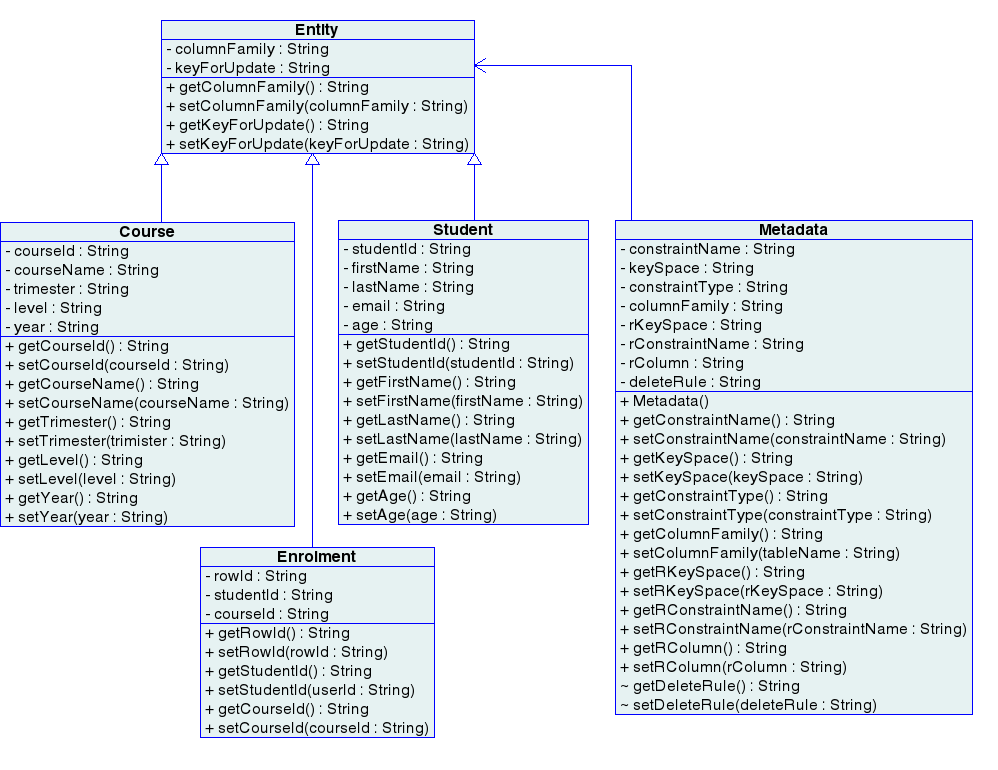
\includegraphics[width=1\textwidth]{./figure/Solutions/classdiagram-experimental.png}
		\caption{Class Diagram for University}\label{fexp:ClassDiagram}
	\end{figure} 

% The constraints for the keyspace are stored in  a  \texttt{Metadata} entity
% class.These constraints are the \ac{PK} and \ac{FK} constraints applicable on each of
% the column families in this keyspace. The list of constraints are the same for
% all the solutions  and are shown in Table~\ref{texp:ListConstraints}.

The list of constraints created for the University keyspace can be seen in
Table~\ref{texp:ListConstraints}. \texttt{CONST100... CONST700} \todo{explain
the purpose of each of them}.


\begin{table}[h] \label{texp:ListConstraints}
\centering
\caption{Metadata}	
	\newcolumntype{C}{@{\hspace{2.5pt}}>{\scriptsize}c@{\hspace{2.5pt}}}
	\begin{tabular}{CCC CCC CC}
		\toprule
		\bfseries ConstraintName & \bfseries Keyspace & \bfseries ConstraintType &
		\bfseries ColumnFamily & \bfseries RKeyspace & \bfseries RConstraintName &
		\bfseries RColumn & \bfseries DeleteRule\\
		\midrule
		CONST100 & University & P & Student & University & & StudentId &\\
		\rc CONST200 & University & P & Course & University & & CourseId &\\
		CONST300 & University & P & Enrolment & University & & RowId &\\
% 		\hline
% 		\hline
		\rc CONST400 & University & R & Enrolment & University & CONST100 & StudentId
		& CASCADE\\
		CONST500 & University & R & Enrolment & University & CONST200 & CourseId &
		NODELETE\\
		\rc CONST600 & University & F & Course & University & CONST500 & CourseId &
		NODELETE\\
		CONST700 & University & F & Student & University & CONST400 & StudentId &
		CASCADE\\
		\bottomrule
	\end{tabular}
\end{table}

% The \texttt{ValidationHandler} in each solution checks these constraints to
% validate referential integrity within this keyspace. The entities are loaded
% generically by the \texttt{EntityManager} for each solution. 
% In the experiment,
% the number of entities inserted for each column family in all the solutions are
% shown in Table~\ref{texp:EntityList}. 
% 	
% 	\begin{table} \label{texp:EntityList}
% 	\centering
% 	\newcolumntype{C} {@{\hspace{2.5pt}}>{\scriptsize}c@{\hspace{2.5pt}}}
% 		\begin{tabular}{CC}
% 			
% 			\toprule
% 			\bfseries ColumnFamily & \bfseries No. of Entities \\
% 			\midrule
% 			Student & 1000 \\
% 			\rc Course & 1000 \\
% 			Enrolment & 10000  \\
% 	% 		\hline
% 	% 		\hline
% 			
% 			\bottomrule
% 		\end{tabular}
% 	\end{table}


\section{Cassandra cluster} \label{sexp:CassandraCluster}
Cassandra is deployed in an homogeneous cluster conformed by 10 nodes. That is,
 all 10 nodes have the same characteristics in software and hardware. These
 nodes emulate a cloud environment in which each node saves
 the data on the local disks of the machines. Notice that, for Solution~4,  an
 additional node is used to emulate an external cluster dedicated to provide
 metadata of the entities upon request.
 The characteristics of these nodes are:


\begin{itemize}
  \item Hardware: \todo{Look on internet the specs of the model}
  	\begin{itemize}
  	  
  	 \end{itemize}
  \item Software: 
  \begin{itemize}
    \item Operating system
    \item Java JDK
    \item Cassandra version 0. 8. 4 
    \item Hector version 0. 8. 0-2.
  \end{itemize}
\end{itemize}


 


% 	\begin{table}[H] \label{texp:Nodeconfig}
% 	\centering
% 	\newcolumntype{C} {@{\hspace{2.5pt}}>{\scriptsize}c@{\hspace{2.5pt}}}
% 		\begin{tabular}{CC}
% 			\toprule
% % 			\bfseries System configurations\\
% 			
% 			Linux kernel version & Linux 3. 2. 4-1-ARCH i686 (62-bit)\\
% 			\rc CPU & Intel(R) Core(TM)2 Duo CPU     E8400  @ 3. 00GHz \\
% 			CPU cores & 4  \\
% 			\rc Network Card & 3 Gigabit \\
% 			Allocated memory & ?? \\
% 			\bottomrule
% 		\end{tabular}
% 	\end{table}

The nodes used in the cluster are part of the \ac{ECS} grid system of
\ac{VUW}. Notice that, such a cluster is not a controlled environment and it is
not possible to use it as  a dedicated cluster as it is also used for other grid
jobs as well as students. Nonetheless, the experiments can be performed over
night during weekends when the external usage of the nodes is minimal.

Some values in the configuration files on each node are changed before starting
the cluster of nodes.  For every node,  the \texttt{listen\_address} and
\texttt{rpc\_address} are set to the hostname.  The nodes are added to the
cluster in a sequential order.  One of the nodes is chosen as the first node and
is made the host node (a.k.a. seed node).  
This node becomes the contact point
for other nodes that join the cluster \todo{? is this true? if it is a ring
topology, then it doesnt sound right, especially after saying later that it
does not contact any other node}.
The list of seed nodes for any given node is specified in a configuration file under the \texttt{seeds} option.  For the
 first node,  this option is set to its loopback address \texttt{127.0.0.1}
 to indicate that it does not contact any other node to join the cluster.  For
 nodes that are not seed nodes, this option contains the hostnames that it can
contact to learn about the cluster.  In the experiments,  except for the first
node, the remaining 9 nodes have two neighboring hosts  as seeds. 

The seed node has its \texttt{auto\_bootstrap} option set to \texttt{true} to
allow other nodes to migrate data from it when data is partitioned or when other
nodes join the cluster.  For nodes that are not seed nodes,  this option is set
to \texttt{false}.  This is because all the nodes are started prior to the 
experiments and do not have data to partition yet. 
 
% The Random Partitioner distributes rows in a cluster evenly and is the
% default configuration setting when Cassandra is installed. 
All the remaining
settings in the Cassandra configuration file are set to the  default values
for all the nodes.  The directories for saving the data,  commit logs and saved
caches are saved on the local disk of each node in its temporary
folder folder (\texttt{/local/tmp}).

% As for Solution~4, an additional node is created to serve as an external
% cluster. 
%  Note that for the Metadata cluster used in Solution~4,  the  cluster
% name is \texttt{MetadataCluster}and the ports for Thrift clients  and TCP sessions are
% changed.  

% Once the cluster is started,  the experiments are initiated and the time taken 
% operations are measured based on performance metrics.  The metrics used for the experiments
% are described in the following section. 


%ब
\section{Experimental setup}\label{sexp:ExperimentalSetup}

The experimentation is based on performing \ac{CRUD} operations upon artificial
data created for the University example application. Since it is not a
controlled environment, the experimentation involves performing several runs
where data is inserted, updated, and deleted on the Cassandra cluster. The
environment is not controlled as variables like network latency, parallel
processes in the nodes, and other variables affect the performance.

On each run,  the time required for each operation is recorded in order to assess
its response time for each solution. Additionally,  

 Notice that, each operation on the
artificial data is performed in a batch,   and entities from each column family
are randomly sorted before any operation takes place.  Random sorting is performed in order to
prevent the results to be biased from possible optimization made by Cassandra in
terms of indexes or other criteria. 
		
The artificial data is made up of  students,   courses,  and 
enrolments which is the result of assigning 10 different courses to each
student.  Courses are assigned by dividing the number of courses
into 100 groups of 10 courses each,  and assigning a group for each student. 
Notice that such an assignment involves that X students have the same courses
assigned.  The quantity of records to be inserted for each entity was chosen
considering an overall reasonable time for completing the experimentation of all
solutions. 
		
The format of the artificial data created is as follows.  
	\begin{itemize}
	  
		  \item \texttt{Student} has a
		unit-increasing \texttt{StudentId},  which is merged into the fields \texttt{FirstName}
		 and \texttt{LastName} as "First Name (StudentId)" and "Last Name
		(StudentId)".  \texttt{Email} is composed in a similar way as
		``First. Last@email. (StudentId). com'' and \texttt{Age} is a random number. 
		
		\item  \texttt{Course} has a unit-increasing \texttt{CourseId} which is
		appended to the prefix "COMP".  It also has a composed \texttt{CourseName} as
		in \texttt{Student} (merging id and field).  \texttt{Trimester},  \texttt{Level}
		and \texttt{Year} are randomly generated numbers. 
		
		\item  \texttt{Enrolment} contains a unit-increasing \texttt{RowId},  and the
		respective foreign keys of student and course,  which are \texttt{StudentId}
		and \texttt{CourseId}. 
		
	\end{itemize}

		
The order of the operations performed on the data is as follows.  \textbf{Create}
inserts all the entities for \texttt{Student},  \texttt{Course} and
\texttt{Enrolment}.  \textbf{Update} performs changes on the primary keys of
students and courses,  and on the foreign keys of \texttt{Enrolment} (the one
relative to courses,  specifically).  Finally,  \textbf{Delete} removes all the
\texttt{Student},  \texttt{Course} and \texttt{Enrolment} entities. 
Notice that the primary keys in every column family are different in each run
(create,  update,  delete) in order to avoid introducing biases to the results as
product of the tombstone delete paradigm that Cassandra utilizes.  That is,  since
Cassandra does not completely  remove the primary keys of the inserted entities
(tombstone delete),  reinsertion  using the same primary key might yield faster
times as the key already exists.  After each run,  all column families
(\texttt{Student},  \texttt{Course},  and \texttt{Enrolment}) are emptied and
ready for the next run.   The details  of the \ac{CRUD} operations are explained
further in the following sections. 
		

	
\subsection{Create} The \texttt{Create} operation inserts all the
\texttt{Student},  \texttt{Course} and \texttt{enrolment} entities in that
precise order due to the nature of the referential integrity constraints
presented in Section~\ref{s:ed:ri}.  The time required to insert all of the
entities in their respective column families  is recorded.  In the
\texttt{Student} and \texttt{Course} column families,  \texttt{Create} does not
trigger any referential integrity validation as these entities do not contain
foreign keys. 
Contrarily,  \texttt{Create} on \texttt{Enrolment} triggers foreign key
validation checks on both \texttt{Student} and \texttt{Course} column families. 
		
\subsection{Update} The \texttt{Update} operation is performed after the
creation of all entities. 
First,  an attempt to update the primary key of each \texttt{Course} entity is
made.  This triggers referential integrity validations that result in exceptions
thrown as the \texttt{DeleteRule} for all \texttt{Course} entities is
\texttt{NoDelete}.  Hence,  the times recorded for updating the \texttt{Course}
column family represent the time required to identify a constraint violation and throw
the respective exceptions. 
					
Next,  the \texttt{Enrolment} column family is updated.  In this case,  the
\texttt{CourseId} for each \texttt{Enrolment} entity is changed to a different
one,  ensuring that the distribution of courses and students remains the same. 
The update on the \texttt{Enrolment} column family triggers referential
integrity validation checks to ensure that the course to which every
\texttt{Enrolment} entity is being updated actually exists in \texttt{Course}
column family. 
					
Finally,  the primary key for each \texttt{Student} entity is updated to a new
integer value that previously  never existed in the column family.  Given the
\texttt{Cascade} \texttt{DeleteRule} for \texttt{Student},  this operation
triggers a cascaded update on the
\texttt{Enrolment} column family.  
%  by respectively updating the student foreign
% key,  \texttt{StudentId} in all its existing \texttt{Enrolment} entities. 
All the dependant \texttt{Enrolment} entities of this \texttt{Student} entity
are respectively updated on its foreign key \texttt{StudentId}. 
		
\subsection{Delete} The deletion of entities occurs first on the
\texttt{Enrolment} column family,  where all of its records are deleted without
requiring referential integrity checks as this is a child entity.  The times are
recorded for each \texttt{Delete} operation and then all of the entities are
reinserted with the same primary keys in order to assess the cascaded delete of
\texttt{Student} entities next. 
				
Secondly,  all  the \texttt{Student} entities are deleted from the
\texttt{Student} column family.  Given the \texttt{Cascade} \texttt{DeleteRule} of these entities,  the
\texttt{ValidationHandler} ensures to delete first all of the child entities
before deleting a \texttt{Student} entity. 
Hence,  the times recorded for this operation measure the time required for
performing a cascaded delete on the student dependencies in enrolment.  Notice
that the dependencies exist at this point as they will have been reinserted into
\texttt{Enrolment} in the previous step. 
				
Finally,  all the \texttt{Course} entities are deleted.  Despite the courses
having a \texttt{NoDelete} rule,  notice that at this point the
\texttt{Enrolment} column family is empty,  so courses can be deleted as there
are no child dependencies.  Thus,  the times recorded for this operation measure
referential integrity validation as well as the \texttt{Delete} operation
of the respective entity.  After this final operation,  all column families are
emptied but all the primary keys still exist due to Cassandra's tombstone
delete.  However,  the whole keyspace is ready for the next batch of operations as
the primary keys of all column families will be different. 
	
	



%ब
\section{Performance Indicators} \label{sexp:PerformanceIndicators}
% Performance of database systems is commonly measured in terms of the
% \textit{Response time} and \textit{Throughput}. 

In this thesis,  response time and throughput are the measures used to gauge the
performance of the four solutions while referential integrity validation is
implemented using the \ac{API}. 
Response time refers to the time  a database system takes to process an
operation and produce results to the end user(\todo{cite Demurjian, 
Berkely, serverside, }).  
% Measuring response time for a
% database operation is similar to a black-box evaluation because it is measured 
% without considering the internal functioning  of the database system.  According
% to (\todo{cite Demurjian}) such an evaluation is ideal for a complete database
% system to measure its performance and to give the users details about its 
% efficiency and speed in performing operations.  
Response time for each of the  operations that trigger such a validation from
all the solutions are measured during the experiments. 
This included the time involved to access and retrieve metadata for the entities
and also the time for validating referential integrity by the
\texttt{ValidationHandler}.  
% The response time of Cassandra when such validations
% are not in place is also measured and considered as a baseline with which to
% analyse the solutions.  Such a comparison determines the degree of change in
% speed of Cassandra when such overheads are introduced and gives users useful
% information about how each solution affects the performance of the database
% system. 

The second performance measure used is \textit{Throughput} which is another
classical and commonly used measure of database performance (\todo{cite
BerkleyDB}).  Throughput measures the number of operations processed by the
database system in a unit of time.  In the experiments the throughput of all the
operations triggering referential integrity validation across all solutions is
measured as operations per second.  A single operation stands for each time an
entity is inserted or updated or deleted. Note that only the operations that
introduce the referential integrity validation are measured and thus
\texttt{read} operations are not measured in terms of response time or
throughput. 

% For example,  inserting 1000 students means that 1000 \texttt{insert}
% operations are processed by Cassandra. 
Notice that external variables such as network latency,  simultaneous processes
in the operating systems of each node,  and other variables are not considered
for the analysis of results.  Even when they are present,  it is expected that
results will not be biased by them.  Nonetheless,  the experiments will be
performed at night time over weekends as this is the time when the cluster is
least used,  thus reducing the presence of such variables and hence their impact
by biasing the results. 

In the experiments,  response time and throughput are measured by logging the
time involved to complete each operation in all the solutions. 
For this,  the  real time is recorded before and after every validation.  When all
the iterations of the experiment are completed,  the time
measurements are written to an output log file. 

The traditional TPC benchmarks are not considered as performance measures in
this experiment  because these benchmarks are centred around transactions and
OLTP workloads.  The principal metrics for these benchmarks are the transaction
rate,  query per hour,  cost indicators of a system,  among others,  which are
suitable indicators for \ac{DBMS} with ACID properties~\citep{TPC}.  Hence,  for
assessing Cassandra which lacks SQL queries and  ACID properties,  these
benchmarks are not suitable indicators of performance. 
%  it is
% essential to measure it in terms of what is critical to application  using Cassandra.  In this experiment it is critical to
% measure the difference in time for an operation to complete in Cassandra when
% referential integrity validation is activated or not activated. 


% These operations which trigger referential integrity validation for an entity
% namely the \texttt{insert},  \texttt{update},  \texttt{delete} operations are
% were measured in terms of the throughput in the experiments.  Throughout
% commonly referes to the number of operations performed

% It has to be noted that the operations are prone to  external factors like
% network latency,  bandwidth,  network routing,  network workload among others
% which typically affect a network consisting of several machines and users. 
% This is because the Cassandra cluster used in the experiments is deployed over
% a network that is used by many users concurrently thus exposing the operations
% to such factors.  Identifying such factors and analysing them is beyond the
% scope of this thesis and the analysis is strictly in terms of how the metadata
% storage and referential integrity validation affects Cassandra's performance. 
% It is a general practise for applications to incorporate code within
% applications to log the timestamps for transactions in traditional
% \acp{DBMS}~\citep{IBMPerformance}. 


% In order to determine the response time and throughput,  the output log files are
% are analysed using R.  (\todo{explain how it is imported to R and graphs
% produced--SOS Juan!})





\section{Summary} \label{sexp:Summary} 

This chapter  presented the experimental design to evaluate the performance of
each  solution and the experimental \ac{API} itself using the prototype keyspace
that is used as an example across this thesis.  The experimental design involves
assessing the performance of the CRUD operations on the different solutions
proposed for referential integrity. 
The analysis of results is to be based on response time and throughput,  two
performance indicators that serve as guidelines for assessing the trade-offs
between the different solutions proposed. 
	
	
The next chapter presents the results and their discussions of the experimental
design presented in this chapter
 






